\documentclass[12pt]{article}

\usepackage[utf8]{inputenc}
\usepackage{datetime}
\usepackage{amsthm}
\usepackage{amsmath}
\usepackage{amssymb}
\usepackage{enumitem}
\usepackage[USenglish]{babel}
\usepackage{matlab-prettifier}
\usepackage{graphicx}
\usepackage[makeroom]{cancel}
\usepackage{afterpage}
\usepackage{capt-of}

\DeclareMathOperator*{\argmin}{arg\,min}

\newcommand\independent{\protect\mathpalette{\protect\independenT}{\perp}}
\def\independenT#1#2{\mathrel{\rlap{$#1#2$}\mkern2mu{#1#2}}}

\newtheoremstyle{colon}{\topsep}{\topsep}{}{}{\bfseries}{:}{ }{}
\theoremstyle{colon}
\newtheorem{exercise}{Exercise}
\newtheorem*{answer}{Answer}

\title{ORFE 525: Statistical Learning and \\ Nonparametric Estimation \\ Homework 2}
\author{Zachary Hervieux-Moore}

\newdate{date}{23}{03}{2017}
\date{\displaydate{date}}

\begin{document}

\maketitle

\clearpage

\begin{exercise}
  This is an effort to reproduce the Moneyball analysis using R.
  \begin{enumerate}[label=\alph*)]
    \item Fit salary by variables on the right of \texttt{POS} using tree regression via \texttt{rpart()}. Compare the mean square errors on the training and testing data separately for the two methods: tree regression with or without pruning. You can choose the parameters of the methods yourself. Plot your fitted trees via \texttt{prp()}.
    \item Fit salary by variables on the right of \texttt{POS} using tree regression via \texttt{randomForest()} with different number of baggings $B$. Plot the mean square errors on the training and testing data separately with $B$ as the x-axis. You canc hoose the other parameters of the methods yourself.
    \item Compare the above two results and which model performs better (in terms of testing error)? Using the better performed model to find the player most undervalued (i.e., the predicted salary has the largest positive gap from the real salary). Check his salary in the following years in \textit{Baseball Prospectus}. As a general manager, what do you think is the possible reasons that he is undervalued.
  \end{enumerate}
\end{exercise}

\clearpage

\begin{answer}
  The code used for this question is appended at the end.

  \begin{enumerate}[label=\alph*)]
    \item The three figures show the tree generated for 3 possible pruning values. Figure 1 is no pruning, Figure 2 is cp = 0.1, and Figure 3 is cp = 0.3. Notice that even with cp = 0.3, the tree reduces down to a single node. The mean square errors are in Table 1.
      \begin{center}
        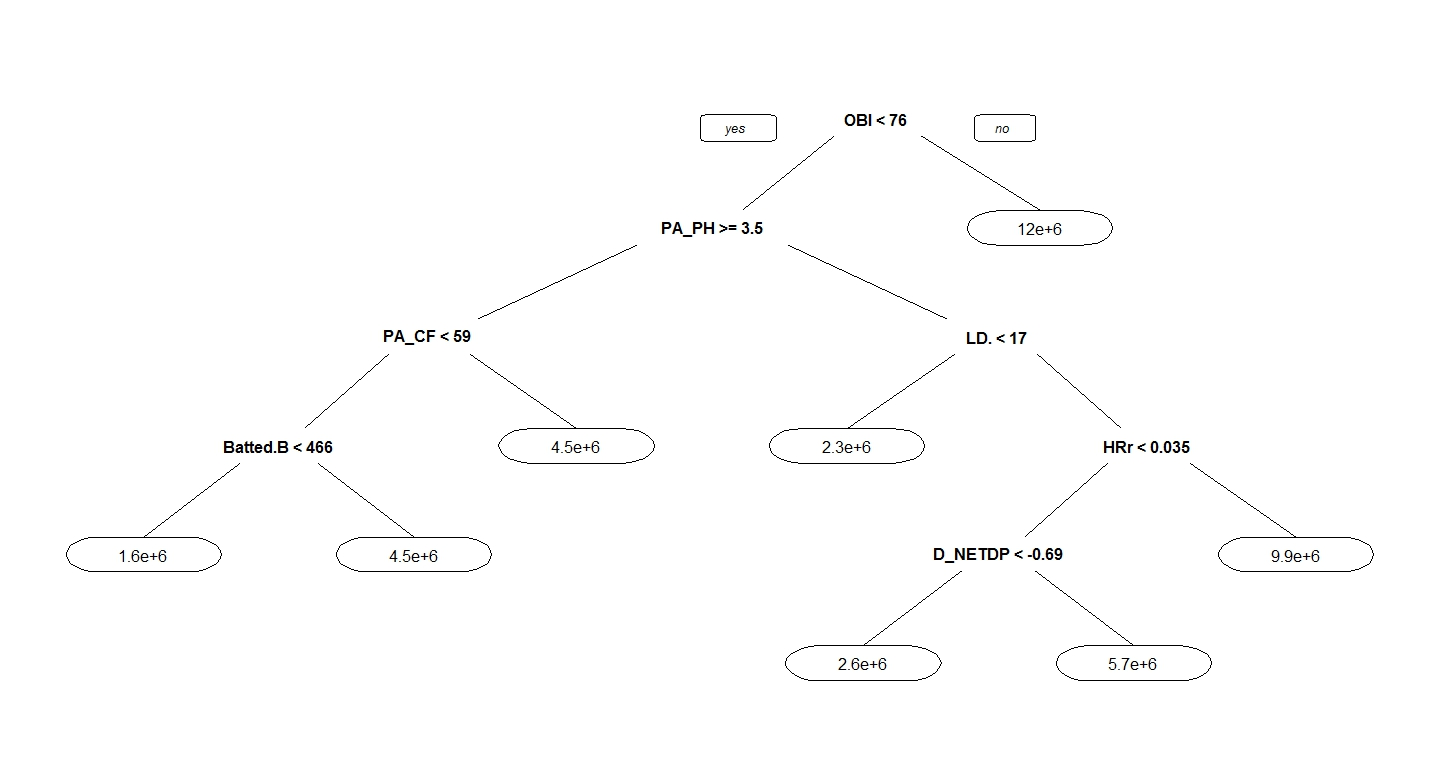
\includegraphics[width=0.9\textwidth]{question1a_no_prune.jpeg}
        \captionof{figure}{Tree with no Pruning}
      \end{center}

      \begin{center}
        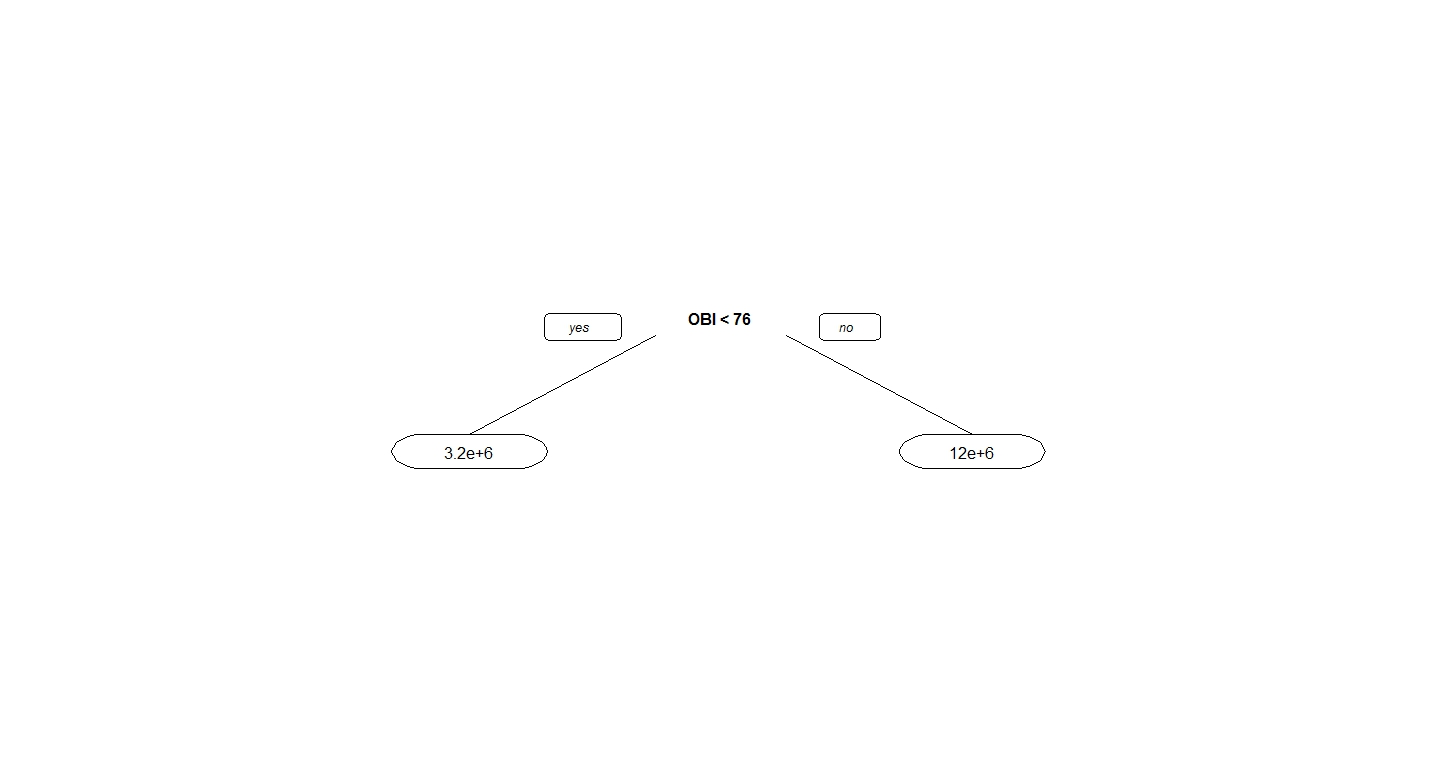
\includegraphics[width=0.9\textwidth]{question1a_0_1.jpeg}
        \captionof{figure}{Tree with cp = 0.1}
      \end{center}

      \begin{center}
        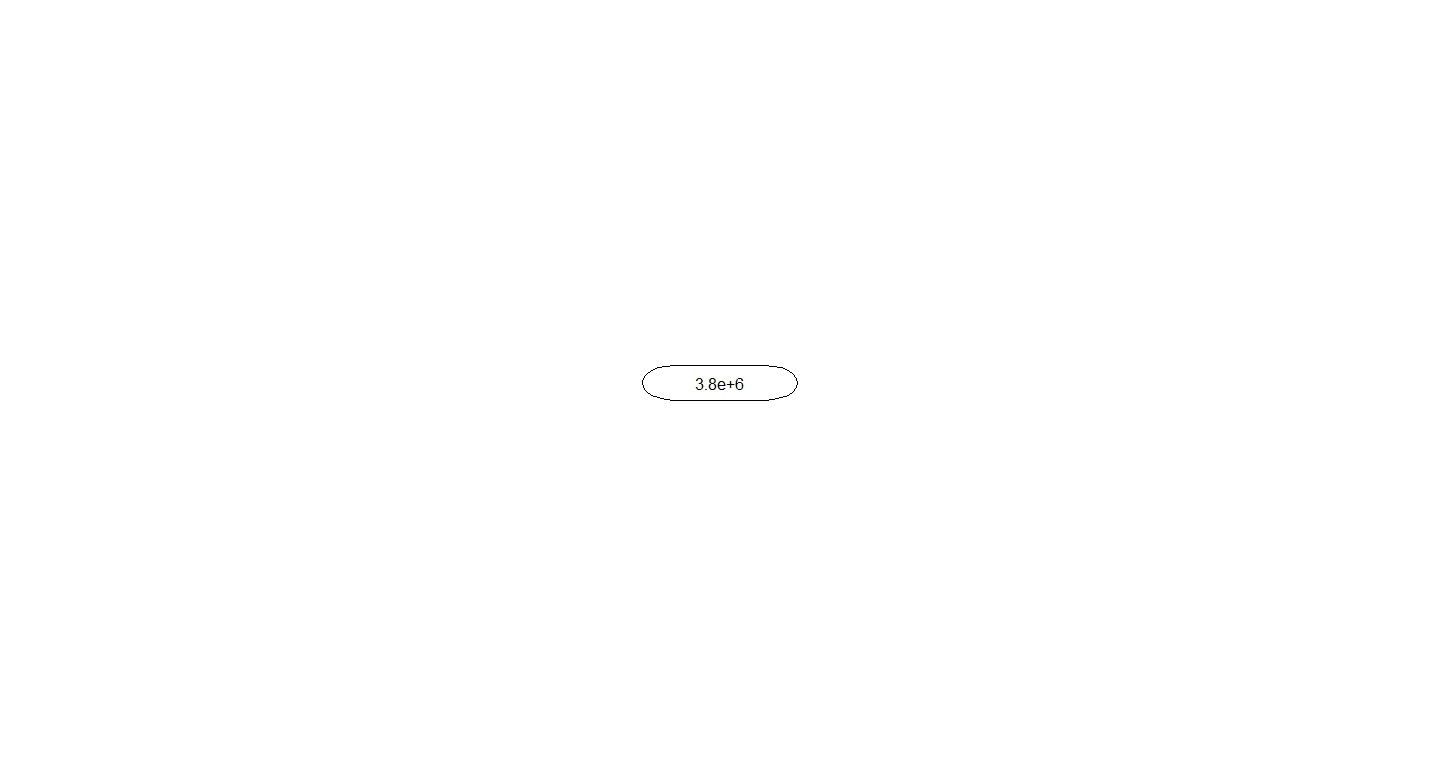
\includegraphics[width=0.9\textwidth]{question1a_0_3.jpeg}
        \captionof{figure}{Tree with cp = 0.3}
      \end{center}

      \begin{center}
        \captionof{table}{MSE Values}
        \begin{tabular}{| c | c | c | c |}
          \hline
          & \text{No pruning} & cp = 0.1 & cp = 0.3 \\
          \hline
          \text{Training Set} & 36198241 & 44735393 & 52769876 \\
          \hline
          \text{Test Set} & 72784943 & 74445712 & 73588157 \\
          \hline
        \end{tabular}
      \end{center}
    \clearpage

    \item Figure 4 shows the MSE values as you vary $B$ from 10 to 200 in increments of 5.
      \begin{center}
        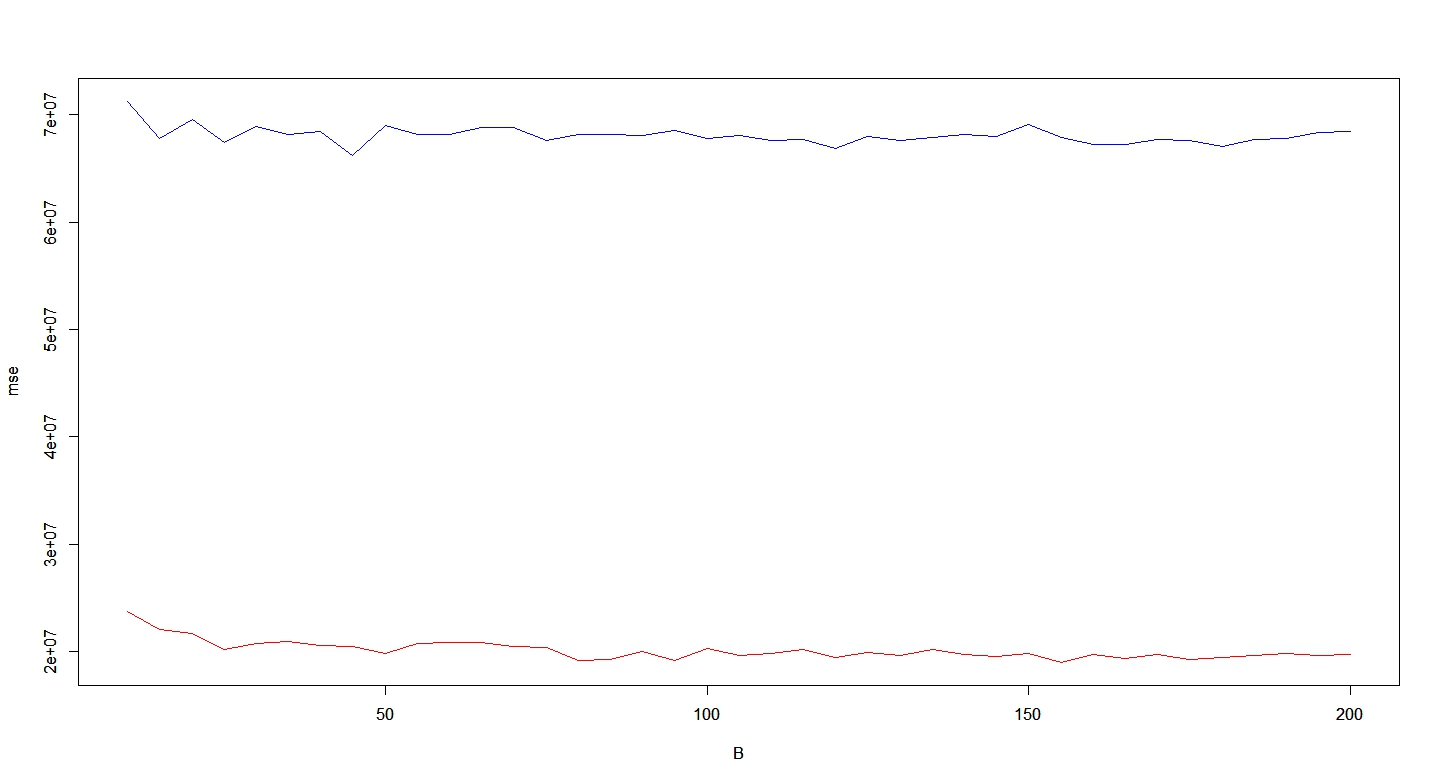
\includegraphics[width=0.9\textwidth]{question1b_mse.jpeg}
        \captionof{figure}{MSE vs. $B$. Blue is test set and red is training set.}
      \end{center}

    \item In terms of testing error, the random forest with $B = 45$ performed the best for me. This yielded that the most undervalued player is Jack Cust with an actual salary of \$410,000, and a predicted salary of \$8,461,580. His salary through the years is shown in Table 2. As a general manager, as you can see that he only lasted 4 years after the 2008 season, the reason why he was undervalued was because he had an anomolous year.
      \begin{center}
        \captionof{table}{Salary of Jack Cust}
        \begin{tabular}{| c | c |}
          \hline
          \text{Year} & \text{Salary} \\
          \hline
          2008 & \$410,000 \\
          \hline
          2009 & \$2,800,000 \\
          \hline
          2010 & \$2,650,000 \\
          \hline
          2011 & \$2,500,000 \\
          \hline
          2012 & \$148,000 \\
          \hline
        \end{tabular}
      \end{center}
  \end{enumerate}

  \textbf{Code Appendix}

  \begin{lstlisting}[language=R, basicstyle=\scriptsize, breaklines=true]
    set.seed(525)

    data <- read.csv("MLB2008.csv")

    data.train <- data[1:154,]
    data.test <- data[155:nrow(data),]

    # Question 1a
    library('rpart')
    library('rpart.plot')

    ## Everything to the right of POS
    x_names <- names(data)[6:134]
    formula <- paste("SALARY ~ ", paste(x_names, collapse= "+"))

    ## No prune
    data.rpart.model <- rpart(formula, data.train)
    dev.new()
    prp(data.rpart.model)

    ## MSE no prune
    data.rpart.train.predict <- predict(data.rpart.model, data.train)
    mse <- norm(data.rpart.train.predict - data.train$SALARY, type="2")
    sprintf("MSE for trained data: %0.0f", mse)

    data.rpart.test.predict <- predict(data.rpart.model, data.test)
    mse <- norm(data.rpart.test.predict - data.test$SALARY, type="2")
    sprintf("MSE for test data: %0.0f", mse)

    ## Prune parameter of 0.1
    data.rpart.prune.model <- prune(data.rpart.model, cp=0.1)
    dev.new()
    prp(data.rpart.prune.model)

    ## MSE no prune
    data.rpart.prune.train.predict <- predict(data.rpart.prune.model, data.train)
    mse <- norm(data.rpart.prune.train.predict - data.train$SALARY, type="2")
    sprintf("MSE for trained data (pruned): %0.0f", mse)

    data.rpart.prune.test.predict <- predict(data.rpart.prune.model, data.test)
    mse <- norm(data.rpart.prune.test.predict - data.test$SALARY, type="2")
    sprintf("MSE for test data (pruned): %0.0f", mse)

    ## Prune parameter of 0.3
    data.rpart.prune.model <- prune(data.rpart.model, cp=0.3)
    dev.new()
    prp(data.rpart.prune.model)

    ## MSE no prune
    data.rpart.prune.train.predict <- predict(data.rpart.prune.model, data.train)
    mse <- norm(data.rpart.prune.train.predict - data.train$SALARY, type="2")
    sprintf("MSE for trained data (pruned): %0.0f", mse)

    data.rpart.prune.test.predict <- predict(data.rpart.prune.model, data.test)
    mse <- norm(data.rpart.prune.test.predict - data.test$SALARY, type="2")
    sprintf("MSE for test data (pruned): %0.0f", mse)

    # Question 1b
    library('randomForest')

    random_forest.mse.train <- data.frame(B=integer(), mse=numeric())
    random_forest.mse.test <- data.frame(B=integer(), mse=numeric())

    for(B in seq(10, 200, by=5)) {
        data.random_forest.model <- randomForest(as.formula(formula), data=data.train, ntree=B)
        df <- data.frame(B, mse=norm(predict(data.random_forest.model, data.train) - data.train$SALARY, type="2"))
        random_forest.mse.train <- rbind(random_forest.mse.train, df)
        df <- data.frame(B, mse=norm(predict(data.random_forest.model, data.test) - data.test$SALARY, type="2"))
        random_forest.mse.test <- rbind(random_forest.mse.test, df)
    }

    dev.new()
    plot(random_forest.mse.train,type="l",col="red", ylim=range(c(random_forest.mse.train["mse"],random_forest.mse.test["mse"])))
    par(new = TRUE)
    plot(random_forest.mse.test,type="l",col="blue", ylim=range(c(random_forest.mse.train["mse"],random_forest.mse.test["mse"])))

    # Question 1c

    ## Min MSE on test data is random forest with B=45 (predict on full data set)
    data.random_forest.model <- randomForest(as.formula(formula), data=data.train, ntree=45)
    data.random_forest.full <- predict(data.random_forest.model, data)

    ## Most undervalued
    data.random_forest.undervalued <- (data.random_forest.full - data$SALARY)
    undervalued <- which.max(data.random_forest.undervalued)
    undervalued.player <- data[c("PLAYER","SALARY")][undervalued,]
    sprintf("Most undervalued player: %s, Actual: $%0.0f, Predicted: $%0.0f", undervalued.player$PLAYER, undervalued.player$SALARY, data.random_forest.undervalued[undervalued])
  \end{lstlisting}
\end{answer}

\clearpage

\begin{exercise}
  In this problem, we will show an insane result in tree regression with categorical variables. We will prove that we can treat categorical variables as if they are ordered (imagine how counterintuitive it is for the zipcode data you used in the last homework).

  Suppose we use the tree regression to fit the data $\{Y_i, X_i\}_{i=1}^n$. Here the predictor $\{X_i\}_{i=1}^n$ are categorical variables having $M$ possible \textbf{unordered} values in $\{1,\mathellipsis,M\}$. In order to minimize the square loss
  \begin{gather*}
    \min_{f \in T_K} \sum_{i=1}^n (Y_i - f(X_i))^2
  \end{gather*}
  where $T_K = \{ f : f(x) = \sum_{k=1}^K \alpha_k I(x \in L_k) \}$ is the tree function class with $K$ leaves and $L_k$ is a leaf. Since $X_i$'s are categorical, the leaves $L_k$'s are $K$-partition of $M$ categories. Namely, $L_k$'s are \textbf{nonempty} and \textbf{disjoint} sets such that $L_1 \cup \mathellipsis \cup L_K = \{1,\mathellipsis,M\}$.

  Let the number of all possible partitions of $\{1,\mathellipsis,M\}$ be $\mathcal{N}_1$. This is a huge number which makes the minimization above intractable. However, we will show in hte problem that the computation can be dramatically simplified by ``pretending'' $X_i$'s to be ordered. Here is how we play the magic. For any $s \in \{1,\mathellipsis,M\}$, without loss of generality, we assume the set $\{X_i = s\}$ is non-empty. Let
  \begin{gather*}
    \bar{Y}_s = \frac{1}{\lvert \{X_i = s\} \rvert} \sum_{X_i = s} Y_i
  \end{gather*}
  Suppose $\bar{Y}_s$ are different for different $s$. Without loss of generality again, we assume that $\bar{Y}_1 < \bar{Y}_2 < \mathellipsis < \bar{Y}_M$.
  \begin{enumerate}[label=\arabic*)]
    \item Prove that for $1 \leq u < v < w \leq M$, if $u,w \in L_k$ for some $k$, then $v \in L_k$ as well.
      (\textbf{Hint:} One possible way is to prove by contradiction. If $u,w \in L_k$ but $v \in L_{k'}$, show that at least one of the following lines is true:
      \begin{gather*}
        \lvert \bar{Y}_v - Avg(L_{k'}) \rvert \geq \lvert \bar{Y}_v - Avg(L_{k}) \rvert \text{ and } \lvert \bar{Y}_v - Avg(L_{k'}) \rvert > 0 \\
        \lvert \bar{Y}_u - Avg(L_k) \rvert \geq \lvert \bar{Y}_u - Avg(L_{k'}) \rvert \text{ and } \lvert \bar{Y}_u - Avg(L_k) \rvert > 0 \\
        \lvert \bar{Y}_w - Avg(L_k) \rvert \geq \lvert \bar{Y}_w - Avg(L_{k'}) \rvert \text{ and } \lvert \bar{Y}_w - Avg(L_k) \rvert > 0
      \end{gather*}
      where $Avg(L_k)$ is the average of the set $\{Y_i : X_i \in L_k\}$. Then show that you can reorganize the partition such that the square loss can be smaller.)

    \item Let $\mathcal{N}_2$ be the number of partitions we need to consider for the minimization above if we have proven Q2.1. Calculate the ratio $\mathcal{N}_2/\mathcal{N}_1$ for $K=2$ and you can see how much we improve.
  \end{enumerate}
\end{exercise}

\begin{answer}
  \leavevmode
  \begin{enumerate}[label=\arabic*)]
    \item Let us rewrite the minimization in terms of $Avg(L_k)$
      \begin{align*}
        &\quad \min_{f \in T_K} \sum_{i=1}^n (Y_i - f(X_i))^2 \\
        &= \min_{f \in T_K} \sum_{i=1}^n Y_i^2 - 2 Y_i f(X_i) + f(X_i)^2 \\
        &= \min_{f \in T_K} \sum_{i=1}^n f(X_i)^2 - 2 Y_i f(X_i) \\
        &= \min_{\alpha_k} \sum_{k=1}^K \sum_{i=1}^n \left( \alpha_k^2 I(X_i \in L_k) - 2 \alpha_k I(X_i \in L_k) Y_i \right) \\
        &= \min_{\alpha_k} \sum_{k=1}^K \sum_{X_i \in L_k} \left( \alpha_k^2 - 2 \alpha_k Y_i \right) \\
        &= \min_{\alpha_k} \sum_{k=1}^K \lvert \{L_k\} \rvert \left( \alpha_k^2 - 2 \alpha_k Avg(L_k) \right)
      \end{align*}
      From here, it is evident that the minimizer is thus $\alpha_k = Avg(L_k)$. Thus, we have that the optimum is
      \begin{align*}
        &\ \sum_{i=1}^n (Y_i - f(X_i))^2 \\
        &= \sum_{k=1}^K \sum_{s \in L_k} \sum_{X_i = s} (Y_i - \alpha_k)^2 \\
        &= \sum_{k=1}^K \sum_{s \in L_k} \sum_{X_i = s} \left((Y_i - \bar{Y}_s)^2 + 2(Y_i - \bar{Y}_s)(\bar{Y}_s - \alpha_k) + (\bar{Y}_s - \alpha_k)^2 \right)
      \end{align*}
      But we have that $\sum_{X_i = s} 2(Y_i - \bar{Y}_s)(\bar{Y}_s - \alpha_k) = 0$ so
      \begin{align*}
        &= \sum_{k=1}^K \sum_{s \in L_k} \sum_{X_i = s} \left((Y_i - \bar{Y}_s)^2 + (\bar{Y}_s - \alpha_k)^2 \right) \\
        &= C(Y_i) + \sum_{k=1}^K \sum_{s \in L_k} \lvert \{X_i = s \} \rvert (\bar{Y}_s - \alpha_k)^2 \\
        &= C(Y_i) + \sum_{k=1}^K \sum_{s \in L_k} \lvert \{X_i = s \} \rvert (\bar{Y}_s - Avg(L_k))^2
      \end{align*}
      Assume that $u,w \in L_k$ and $v \in L_{k'}$. We have that $Avg(L_k) \neq Avg(L_{k'})$ since this implies that $\alpha_k = \alpha_{k'}$ and so $L_k$ and $L_{k'}$ are not disjoint. WLOG, let $Avg(L_k) < Avg(L_{k'})$. Now we treat three cases.

      Case 1, $Avg(L_k) < Avg(L_{k'}) \leq \bar{Y}_v$. Since $\bar{Y}_w > \bar{Y}_v$, we have
      \begin{gather*}
        0 < \bar{Y}_w - Avg(L_{k'}) < \bar{Y}_w - Avg(L_k) \\
        \implies \lvert \bar{Y}_w - Avg(L_{k'}) \rvert  < \lvert \bar{Y}_w - Avg(L_k) \rvert
      \end{gather*}
      Which contradicts the optimality of $\alpha_k$.

      Case 2, $Avg(L_k) \leq \bar{Y}_v < Avg(L_{k'})$. If $Avg(L_{k'}) < \bar{Y}_w$ then we get the same as above. Otherwise we have, $Avg(L_{k'}) \geq \bar{Y}_w$. By optimality of $Avg(L_{k'}$
      \begin{gather*}
        \bar{Y}_v - Avg(L_k) \geq Avg(L_{k'}) - \bar{Y}_v \\
        2 \bar{Y}_v \geq Avg(L_{k'}) + Avg(L_k)
      \end{gather*}
      But by assumption and optimality of $Avg(L_k)$
      \begin{gather*}
        2 \bar{Y}_w \leq Avg(L_{k'}) + Avg(L_k)
      \end{gather*}
      Which is a contradiction that $\bar{Y}_w > \bar{Y}_v$.

      Case 3, $\bar{Y}_v < Avg(L_k) < Avg(L_{k'})$
      \begin{gather*}
        0 < Avg(L_k) - \bar{Y}_v < Avg(L_{k'}) - \bar{Y}_v \\
        \implies \lvert Avg(L_k) - \bar{Y}_v \rvert < \lvert Avg(L_{k'}) - \bar{Y}_v \rvert
      \end{gather*}
      which contradicts the optimality of $Avg(L_{k'})$. This handles the three cases and so we conclude that $v \in L_k$ as well.

    \item $\mathcal{N}_1 = 2^M - 1$ since that is how many non-empty partitions are possible. Since $K=2$, we have that $\mathcal{N}_2 = M - 1$ since we only have to consider partitions that have the property $1 \leq u < v < w \leq M$, if $u,w \in L_k$ for some $k$, then $v \in L_k$ as well. This can be seen by the fact that when $K=2$, we must divided $\{1,\mathellipsis,M\}$ into two sets with the largest element of the first set smaller than the least element of the second set. That is, they are of the form $\{1,\mathellipsis,i\}$ and $\{i+1, \mathellipsis,M\}$. There are only $M-1$ choices for $i$. Thus, the ratio is $\mathcal{N}_2/\mathcal{N}_1=\frac{M-1}{2^M-1}$.
  \end{enumerate}
\end{answer}

\clearpage

\begin{exercise}
  In the problem, we will provide a theoretical justification of the dropout trick we learned in depp learning lectures. We will show that dropout is essentially a regularization. This problem also gives us a new statistical method to implement regularization.

  Consider the generalized linear models (GLMs), which defines a conditional distribution over a response $y \in \mathcal{Y}$ given an input feature vecture $x \in \mathbb{R}$.
  \begin{gather*}
    p_\beta (y | x) := h(y) e^{y \cdot x^T \beta - A(x^T \beta)}
  \end{gather*}
  Here $h(y)$ is a quantity independent of $x$ and $\beta$, $A(\cdot)$ is the log-partition function which makes $p_\beta (y | x)$ a valid conditional distribution. Define the negative log-likelihood to be $\ell_{x,y}(\beta) := -\log p_\beta (y | x)$. Instead of $x_i$, we consider the noisy version $\tilde{x}_i = \nu (x_i, \xi_i)$, where two types of noise are considered:
  \begin{itemize}
    \item \textbf{Additive Gaussian noise:} $\nu(x_i, \xi_i) = x_i = \xi_i$, where \\ $\xi_i \sim \mathcal{N}(0, \sigma^2 I_{d \times d})$
    \item \textbf{Dropout noise:} $\nu(x_i, \xi_i) = x_i \odot \xi_i$, where $\odot$ is the element-wise product of two vectors and each component of $\xi_i$ is an independent Bernoulli draw, i.e. $\xi_{ij} = 1 / (1 - \delta)$ with probability $1 - \delta$ and 0 otherwise for $1 \leq j \leq d$.
  \end{itemize}
  Integrating over the feature noise gives us a noised maximum likelihood parameter estimate:
  \begin{gather*}
    \hat{\beta} := \argmin_{\beta \in \mathbb{d}} \sum_{i=1}^n \mathbb{E}_{\xi} [\ell_{\tilde{x}_i, y_i} (\beta)]
  \end{gather*}
  where the expectation $\mathbb{E}_{\xi}[\cdot]$ is taken with respect to $\xi = (\xi_1, \mathellipsis, \xi_n)$ only.
  \begin{enumerate}[label=\arabic*)]
    \item Prove that as long as $\mathbb{E}[\tilde{x}] = x$, we have $\sum_{i=1}^n \mathbb{E}_\xi [\ell_{\tilde{x}_i, y_i}(\beta)]$ \\   $= \sum_{i=1}^n \ell_{x_i, y_i}(\beta) + R(\beta)$, where
    \begin{gather*}
      R(\beta) = \sum_{i=1}^n \left( \mathbb{E}[A(\tilde{x}_i^T \beta)] - A(x_i^T \beta) \right)
    \end{gather*}
    \item If $\mathbb{E}_\xi [\tilde{x}] = x$ and $A'''$ is bounded, show that
      \begin{gather*}
        \mathbb{E}_\xi [A(\tilde{x}^T \beta)] - A(x^T \beta) = \frac{1}{2} A''(x^T \beta) Var_\xi (\tilde{x}^T \beta) + O(\mathbb{E}_\xi [\lvert (\tilde{x} - x)^T \beta \rvert^3])
      \end{gather*}
    \item Define $R^q (\beta) := \frac{1}{2} \sum_{i=1}^n A'' (x_i^T \beta) Var_\xi (\tilde{x}_i^T \beta)$, show that in the linear regression setting, we have
      \begin{itemize}
        \item $R^q (\beta) = \frac{1}{2} \sigma^2 n \lVert \beta \rVert_2^2$ when using the additive Gaussian noise,
        \item $R^q (\beta) = \frac{1}{2} \frac{\delta}{1-\delta} \beta^T \text{diag}(X^T X) \beta$ using dropout noise, where $X \in \mathbb{R}^{n \times d}$ is the design matrix.
      \end{itemize}
  \end{enumerate}
\end{exercise}

\begin{answer}
  \leavevmode
  \begin{enumerate}[label=\arabic*)]
    \item We have that
      \begin{align*}
        &\ \sum_{i=1}^n \mathbb{E}_\xi [\ell_{\tilde{x}_i, y_i}(\beta)] \\
        &= \sum_{i=1}^n \mathbb{E}_\xi [-\log p_\beta (y_i | \tilde{x}_i)] \\
        &= -\sum_{i=1}^n \mathbb{E}_\xi [\log \left( h(y_i) e^{y_i \cdot \tilde{x}_i^T \beta - A(\tilde{x}_i^T \beta)} \right)] \\
        &= -\sum_{i=1}^n \left( \log h(y_i) + \mathbb{E}_\xi [y_i \cdot \tilde{x}_i^T \beta] - \mathbb{E}_\xi [A(\tilde{x}_i^T \beta) \right)] \\
        &= -\sum_{i=1}^n \left( \log h(y_i) + y_i \cdot \mathbb{E}_\xi [\tilde{x}_i^T] \beta - A(x_i^T \beta) \right) + A(x_i^T \beta) - \mathbb{E}_\xi [A(\tilde{x}_i^T \beta)] \\
        &= -\sum_{i=1}^n \left( \log h(y_i) + y_i \cdot x_i^T \beta - A(x_i^T \beta) \right) + \sum_{i=1}^n \left( \mathbb{E}_\xi [A(\tilde{x}_i^T \beta)] - A(x_i^T \beta) \right) \\
        &= \sum_{i=1}^n \ell_{x_i, y_i}(\beta) + R(\beta)
      \end{align*}

    \item We do a Taylor expansion of $A$ at $x \beta$
      \begin{gather*}
        A(\tilde{x}^T \beta) \\
        = A(x^T \beta) + A'(x^T \beta) (\tilde{x} - x)^T \beta + \frac{1}{2} A''(x^T \beta) \beta^T (\tilde{x} - x)^2 \beta + O(\lvert (\tilde{x} - x)^T \beta \rvert^3)
      \end{gather*}
      Taking expectations and recalling that $x$ is not random
      \begin{align*}
        \mathbb{E}_\xi [A(\tilde{x}^T \beta)] &= \mathbb{E}_\xi [A(x^T \beta)] + \mathbb{E}_\xi [A'(x^T \beta) (\tilde{x} - x)^T \beta] \\
        &+ \frac{1}{2} \mathbb{E}_\xi [A''(x^T \beta) \beta^T (\tilde{x} - x)^2 \beta] \\
        &+ O(\mathbb{E}_\xi [\lvert (\tilde{x} - x)^T \beta \rvert^3]) \\
        \mathbb{E}_\xi [A(\tilde{x}^T \beta)] &= A(x^T \beta) + A'(x^T \beta) \mathbb{E}_\xi [ (\tilde{x} - x)^T ] \beta \\
        &+ \frac{1}{2} A''(x^T \beta) \mathbb{E}_\xi [ \beta^T (\tilde{x} - \mathbb{E}_\xi[x])^2 \beta] \\
        &+ O(\mathbb{E}_\xi [\lvert (\tilde{x} - x)^T \beta \rvert^3]) \\
        \mathbb{E}_\xi [A(\tilde{x}^T \beta)] - A(x^T \beta) &= \frac{1}{2} A''(x^T \beta) Var(\tilde{x}^T \beta) + O(\mathbb{E}_\xi [\lvert (\tilde{x} - x)^T \beta \rvert^3])
      \end{align*}
      Where the first derivative term disappears because $\mathbb{E}_\xi [\tilde{x}] = x$.

    \item Since we are in the linear regression setting, we have that $y_i \sim \mathcal{N}(0,1)$. So $A(x_i^T \beta) = (x_i^T \beta)^2/2$. So $A''(x^T \beta) = 1$. Now, let us compute the variance for the two settings. For additive Gaussian noise:
      \begin{align*}
        Var_\xi (\tilde{x}_i^T \beta) &= \beta^T Var_\xi (x_i^T + \xi_i) \beta \\
        &= \beta^T Var_\xi (\xi_i) \beta \\
        &= \beta \sigma^2 I_{d \times d} \beta \\
        &= \sigma^2 \lVert \beta \rVert_2^2 \\
      \end{align*}

      Where the second line is from the fact that $x_i$ is fixed. For dropout:

      \begin{align*}
        \sum_{i=1}^d Var_\xi (\tilde{x}_i^T \beta) &= \sum_{i=1}^d \beta^T Var_\xi (x_i^T \odot \xi_i) \beta \\
        &= \sum_{i,j=1}^d \beta_j Var_\xi (x_{i_j} \cdot \xi_{i_j}) \beta_j = \sum_{i,j=1}^d \beta_j x_{i_j}^2 Var_\xi (\xi_{i_j}) \beta_j \\
        &= \sum_{i,j=1}^d \beta_j x_{i_j}^2 \left(\frac{1}{1-\delta} - 1 \right) \beta_j = \frac{\delta}{1-\delta} \sum_{i,j=1}^d \beta_j x_{i_j}^2 \beta_j \\
        &= \frac{\delta}{1-\delta} \beta^T \text{diag}(X^T X) \beta \\
      \end{align*}

      Where we use the fact that the Bernoulli's are independent to ignore the cross variance terms on the second line. We conclude that
        \begin{gather*}
        R^q (\beta) = \frac{1}{2} \sigma^2 n \lVert \beta \rVert_2^2
        \end{gather*}
      for additive Gaussian noise and
        \begin{gather*}
          R^q (\beta) = \frac{1}{2} \frac{\delta}{1-\delta} \beta^T \text{diag}(X^T X) \beta
        \end{gather*}
      for dropout.
  \end{enumerate}
\end{answer}

\clearpage

\begin{exercise}
  In this problem, we will explore the properties of RIP. We say a matrix $A$ is restricted isometry for $s$, if there exists $\delta \in [0,1)$, such that
  \begin{gather*}
    (1-\delta_s) \lVert x \rVert_2^2 \leq \lVert A x \rVert_2^2 \leq (1+\delta_s) \lVert x \rVert_2^2
  \end{gather*}
  for any $\lVert x \rVert_0 \leq s$, where $\lVert x \rVert_0 = \lvert \text{supp}(x)\rvert$.
  \begin{enumerate}[label=\arabic*)]
    \item For any $1 \leq s \leq d$, the matrix $A \in \mathbb{R}^{m \times d}$ satisfies the RIP with parameter $\delta$. Prove that
      \begin{gather*}
        \lvert \langle Ax, Ay \rangle \rvert \leq \delta_{s+t} \lVert x \rVert_2 \lVert y \rVert_2
      \end{gather*}
      for any $\lVert x \rVert_0 \leq s$, $\lVert y \rVert_0 \leq t$ and $x,y$ have disjoint supports (\textbf{Hint:} Use the polarization identity).

    \item In the class, we show the perfect recovery of compressed sensing under $3s$-RIP condition. In this problem, we will improve the result. We will show that $2s$-RIP is actually enough for perfect recovery. In specific, prove that if $X$ satisfies $2s$-RIP with $\delta_{2s} \leq 1/(1+\sqrt{2})$ and $\lVert \beta^* \rVert_0 \leq s$, then $\hat{\beta} = \beta^*$ where
      \begin{gather*}
        \hat{\beta} = \argmin_{\beta} \lVert \beta \rVert_1 \text{ s.t. } X \beta^* = X \beta
      \end{gather*}
      Think about why we did not get a sharp result in the class?

      (\textbf{Hint:} Instead of dividing the $h = \hat{\beta} - \beta^*$ into parts $S^*, S_1, S_2, \mathellipsis$ of sizes $2s$ in the class, try $s$. Then show $\lVert h_{S^*} \rVert_1 \leq \rho \lVert h_{S^{*^c}} \rVert_1$ for some $\rho < 1$ by starting with
      \begin{gather*}
        \lVert X h_{S^* \cup S_1} \rVert_2^2 = - \sum_{j \geq 2} \langle X h_{S^* \cup S_1}, X h_{S_j} \rangle
      \end{gather*}
      and apply Q4.1).

    \item In the class, we show a sufficient condition for the RIP condition. This problem will give a lower bound of samples needed for the RIP condition. Suppose $A \in \mathbb{R}^{n \times d}$ satisfy RIP with $\delta_{2s} \in (0,1/2]$. Prove that
      \begin{gather*}
        n \geq C s \log \left( \frac{d}{s} \right)
      \end{gather*}
      for some constant $C$ independent of $d$, $n$, and $s$. You can prove this problem following the steps below.

      \textbf{Step 1:} Let $s$ and $d$ satisfying $s < d/2$ be given. Prove that there exists a set
      \begin{gather*}
        \mathcal{X} \subseteq U = \{x \in \{0,+1,-1\}^d : \lVert x \rVert_0 = s\}
      \end{gather*}
      such that for any $x,z \in \mathcal{X}$ with $x \neq z$ we have
      \begin{gather*}
        \lVert x - z \rVert_2 \geq \sqrt{s/2} \text{ and } \log \lvert \mathcal{X} \rvert \geq \frac{s}{2} \log \left( \frac{d}{s} \right)
      \end{gather*}
      You can construct your set by adding points in $U$ one by one and make sure there are points $z$'s that have not been added so far satisfying $\lVert x - z \rVert_2 \geq \sqrt{s/2}$ for $x$'s that have already been added. You need to bound the number of these possible $z$'s if $m$ of $x$'s have been added until you find that it is impossible to find another such $z$. Then you can find the lower bound of $\lvert \mathcal{X} \rvert$.

      \textbf{Step 2:} For any pair of $x,z \in \mathcal{X}$, the balls centered at $Ax, Az$ with radius $\sqrt{s/16}$ are disjoint.

      \textbf{Step 3:} Prove the problem using Step 1 and Step 2. (\textbf{Hint:} Find a larger ball containing all balls in Step 2. Use the fact that the volume of this larger ball is bigger than the sum of the smaller balls in Step 2.)

    \item Let $X \in \mathbb{R}^{n \times d}$. Here we consider three different methods for generating $X$: i.i.d. Gaussian (via \texttt{Gaussian\_Phi.m}), random rows of a discrete cosine transform (via \texttt{SubDCT\_Phi.m}), and consecutive rows of a random Toeplitz matrix (via \texttt{SubToep\_Phi.m}). Let $\beta$ be a vector s.t. $\lVert \beta \rVert_0 = s$ and $Y = X \beta$. Define the compressed sensing estimator
      \begin{gather*}
        \hat{\beta} = \argmin_\beta \lVert \beta \rVert_1, \text{ s.t. } Y = X \beta
      \end{gather*}

      You can solve the prboblem via \texttt{l1eq\_pd.m}. In each of these three cases, set $d=1024$ and use simulation to determine values of $n$ and $s$ such that we can recover the true $\beta$. (You can create sparse vectors $\beta$ at random for the simulation using any distribution you find reasonable). In specific, for each pair of $(n,s)$, use Monte Carlo methods to calculate the probability that the true $\beta$ is recoverd.

      You can visualize your results using a plot where the x-axis is $s/d$ and y-axis is $n/d$ and the rainbow color represents the probability for exact recovery. Do your plots imply some connection to Q4.3 and random matrix theory for RIP? (This is an open question and you can explore as much as possible).
  \end{enumerate}
\end{exercise}

\begin{answer}
  \leavevmode
  \begin{enumerate}[label=\arabic*)]
    \item Since $x$ and $y$ have disjoint supports we have that
      \begin{gather*}
        \lVert x \pm y \rVert_2^2 = \lVert x \rVert_2^2 + \lVert y \rVert_2^2 \\
        \lVert x \pm y \rVert_0 = \lVert x \rVert_0 + \lVert y \rVert_0 \leq s + t
      \end{gather*}
      This gives us the restricted isometry inequalties
      \begin{gather*}
        (1-\delta_{s+t})\lVert x \pm y \rVert_2^2 \leq \lVert Ax \pm Ay \rVert_2^2 \leq (1+\delta_{s+t})\lVert x \pm y \rVert_2^2
      \end{gather*}
      Now we use the polarization identity coupled with the above to get
      \begin{gather*}
        \langle Ax, Ay \rangle = \frac{1}{4} (\lVert Ax + Ay \rVert_2^2 - \lVert Ax - Ay \rVert_2^2) \\
        \langle Ax, Ay \rangle \leq \frac{1}{4} ((1+\delta_{s+t})\lVert x + y \rVert_2^2 - (1-\delta_{s+t})\lVert x - y \rVert_2^2) \\
        \lvert \langle Ax, Ay \rangle \rvert \leq \frac{1}{2} \delta_{s+t} (\lVert x \rVert_2^2 + \lVert y \rVert_2^2)
      \end{gather*}
      Now we use the fact that we can assume that $x$ and $y$ have the same 2 norm without loss of generality (since we can just divide the above inequality by $\lVert x \rVert_2 \lVert y \rVert_2$) to get the result $\lvert \langle Ax, Ay \rangle \rvert \leq \delta_{s+t} \lVert x \rVert_2 \lVert y \rVert_2$.

    \item We follow the hint and the class proof for $3s$-RIP. From class, the proof that $\lVert h_{S^{*^c}} \rVert_1 \leq \lVert h_{S^*} \rVert_1$ is unchanged. Now, we divide $h = \hat{\beta} - \beta$ into parts $S_0 = S^*$, $S_1 = $ locations of $s$-largest entries in $h_{S^{*^c}}$, $S_2 = $ next $s$ largest locations, etc. Then we have
      \begin{gather*}
        \lVert X h_{S^* \cup S_1} \rVert_2^2 = - \sum_{j \geq 2} \langle X h_{S^* \cup S_1, X H_{S_j}} \rangle \\
        \Longleftrightarrow \lVert X h_{S^* \cup S_1} \rVert_2^2 \leq \sum_{j \geq 2} \lvert \langle X h_{S^* \cup S_1}, X H_{S_j} \rangle \rvert
      \end{gather*}
      We now upper bound the right hand side using Q4.1 and lower bound the LHS using $2s$-RIP
      \begin{gather*}
        (1-\delta_{2s}) \lVert h_{S^* \cup S_1} \rVert_2^2 \leq \sum_{j \geq 2} \delta_{s+s} \lVert h_{S^* \cup S_1} \rVert_2 \lVert h_{S_j} \rVert_2 \\
        \Longleftrightarrow \lVert h_{S^* \cup S_1} \rVert_2 \leq \frac{\delta_{2s}}{1-\delta_{2s}} \sum_{j \geq 2} \lVert h_{S_j} \rVert_2
      \end{gather*}
      Now, we upper and lower bound the 2 norms. Lower bound first
      \begin{gather*}
        \lVert h_{S^* \cup S_1} \rVert_2 \geq \lVert h_{S^*} \rVert_2 \geq \frac{\lVert h_{S^*} \rVert_1}{\sqrt{s}}
      \end{gather*}
      Now upper bound
      \begin{gather*}
         \frac{\delta_{2s}}{1-\delta_{2s}} \sum_{j \geq 2} \lVert h_{S_j} \rVert_2 \leq \frac{\delta_{2s}}{1-\delta_{2s}} \sum_{j \geq 2} \sqrt{s} \lVert h_{S_j} \rVert_\infty \leq \frac{\delta_{2s}}{1-\delta_{2s}} \sum_{j \geq 2} \frac{\lVert h_{S_j} \rVert_1}{\sqrt{s}}
      \end{gather*}
      So we conclude
      \begin{gather*}
        \frac{\lVert h_{S^*} \rVert_1}{\sqrt{s}} \leq \frac{\delta_{2s}}{1-\delta_{2s}} \sum_{j \geq 2} \frac{\lVert h_{S_j} \rVert_1}{\sqrt{s}} \\
        \implies \lVert h_{S^*} \rVert_1 \leq \frac{\delta_{2s}}{1-\delta_{2s}} \lVert h_{S^{*^c}} \rVert_1
      \end{gather*}
      Where $\rho = \frac{\delta_{2s}}{1-\delta_{2s}} < 1$ by the conditions on $\delta_{2s}$.

    \item Let us show that one needs $n \geq C s \log \left( \frac{d}{s} \right)$ samples for the RIP condition.

      \textbf{Step 1:} First, since $\mathcal{X} \subseteq U$, we have that $\lvert \mathcal{X} \rvert \leq \lvert U \rvert$. So, we must find a way to lower ound $\lvert \mathcal{X} \rvert$. Let $\mathcal{X}$ be a subset of $U$ with $\lVert x - z \rVert_2 \geq \sqrt{s/2}$ for $x,z \in \mathcal{X}$. Such a set exists because one can take a single point. Take $\mathcal{X}$ to be the largest possible set. Thus, we have $U = \cup_{x \in \mathcal{X}} B_x(\sqrt{s/2})$. Where $B_x(\sqrt{s/2})$ is the ball around $x$ of radius $\sqrt{s/2}$. Thus,
      \begin{gather*}
        \lvert U \rvert \leq \sum_{x \in \mathcal{X}} \lvert B(x, \sqrt{s/2}) \rvert \leq \lvert \mathcal{X} \rvert \lvert B_0(\sqrt{s/2}) \rvert
      \end{gather*}
      Where the above can be visualized that we have points in $\mathcal{X}$ and that all the balls of radius $\sqrt{s/2}$ around these points contain $U$ by definition. Furthermore, the ball centered at 0 contains the most points in $U$ and so we can upper bound any ball with this one. Now, we have
      \begin{gather*}
        \lvert B_0(\sqrt{s/2}) \rvert = \lvert \{ y \in U : \lVert 0 - y \rVert_2 \leq \sqrt{s/2} \} \rvert \\
        \leq \lvert \{ y \in U : \lVert y \rVert_0 \leq \sqrt{s/2} \} \rvert = \binom{d}{\frac{s}{2}} 3^{\frac{s}{2}}
      \end{gather*}
      But we also have that the total points in $U$ is $\binom{d}{s} 2^s$. This is due to the fact that there must be $s$ non zero entries and you have a choice of $\pm 1$ for these points. Thus, putting these together,
      \begin{gather*}
        \lvert \mathcal{X} \rvert \geq \left( \frac{4}{3} \right)^{\frac{s}{2}} \frac{\binom{d}{s}}{\binom{d}{\frac{s}{2}}} \\
        \implies \lvert \mathcal{X} \rvert \geq \left( \frac{4}{3} \right)^{\frac{s}{2}} \frac{(d/s)^s}{(2d/s)^{s/2}} \\
        \implies \lvert \mathcal{X} \rvert \geq \left( \frac{2}{3} \right)^{\frac{s}{2}} (d/s)^{s/2} \\
        \implies \log \lvert \mathcal{X} \rvert \geq \frac{s}{2} \log(2/3) + \frac{s}{2} \log \left( \frac{d}{s} \right) \\
        \implies \log \lvert \mathcal{X} \rvert \geq \frac{s}{2} \log \left( \frac{d}{s} \right)
      \end{gather*}

      \textbf{Step 2:} We have that $x, z \in \mathcal{X}$ then $\lVert x - z \rVert_2 \geq \sqrt{s/2}$ and $\lVert x - z \rVert_0 \leq 2s$. That is, we can use the results from Q4.1 to get
      \begin{gather*}
        \lVert Ax - Az \rVert_2^2 \geq (1-\delta_{2s}) \lVert x - z \rVert_2^2 \geq  (1-\delta_{2s}) \frac{s}{2} \geq \frac{s}{4}
      \end{gather*}
      Where we $\delta_{2s} \in [0,1/2]$ by assumption. Thus, we have that $Ax$ and $Az$ are separated by more than $\sqrt{s/4}$ and we conclude that this is twice the radii.

      \textbf{Step 3:} We wish to contain all the disjoint balls in Step 2. Thus, we use that for $x \in U$ thath $\lVert Ax \rVert_2^2 \leq (1+\delta_{s}) \lVert x \rVert_2^2 \leq \frac{3}{2} \lVert x \rVert_0 = \frac{3}{2}s$. Thus, to contain the balls in Step 2, we must add $1/4 \sqrt{s}$ to the radius of the ball centered at the origin with radius $\sqrt{3/2} \sqrt{s}$. Thus, the larger ball is centered at the origin with radius $(\sqrt{25s/16}$. Now we have that the sum of the small balls in Step 2 is less than the volume of this larger ball
      \begin{gather*}
        \sum_{x \in \mathcal{X}} Vol(\sqrt{s/16}) \leq Vol(\sqrt{25s/16}) \\
        \implies \lvert \mathcal{X} \rvert \sqrt{s/16}^n Vol(1) \leq \sqrt{25s/16}^n Vol(1) \\
        \implies \frac{s}{2} \log\left( \frac{d}{s} \right) \leq n \log(5) \\
        \implies s \log\left( \frac{d}{s} \right) \leq n \log(25) \\
        \implies C s \log\left( \frac{d}{s} \right) \leq n
      \end{gather*}

    \item For computation reasons, I have restricted $d$ to 512 and used a step size of $50$ for $n$ and $s$. Also, 10 iterations of Monte Carlo was done. The figures below show the probabilities for the different random matrices. The x-axis is $s/d$, y-axis is $n/d$, and red is probability 1, blue is probability 0. Note that the y-axis is inverted. You can see the relation to question Q4.3 since $\frac{n}{d} \geq C \frac{s}{d} \log \left( \frac{s}{d} \right)$ for the RIP condition and compare that to the frontier where the probabilities transition from 0 to 1. The code is appended below.

      \begin{center}
        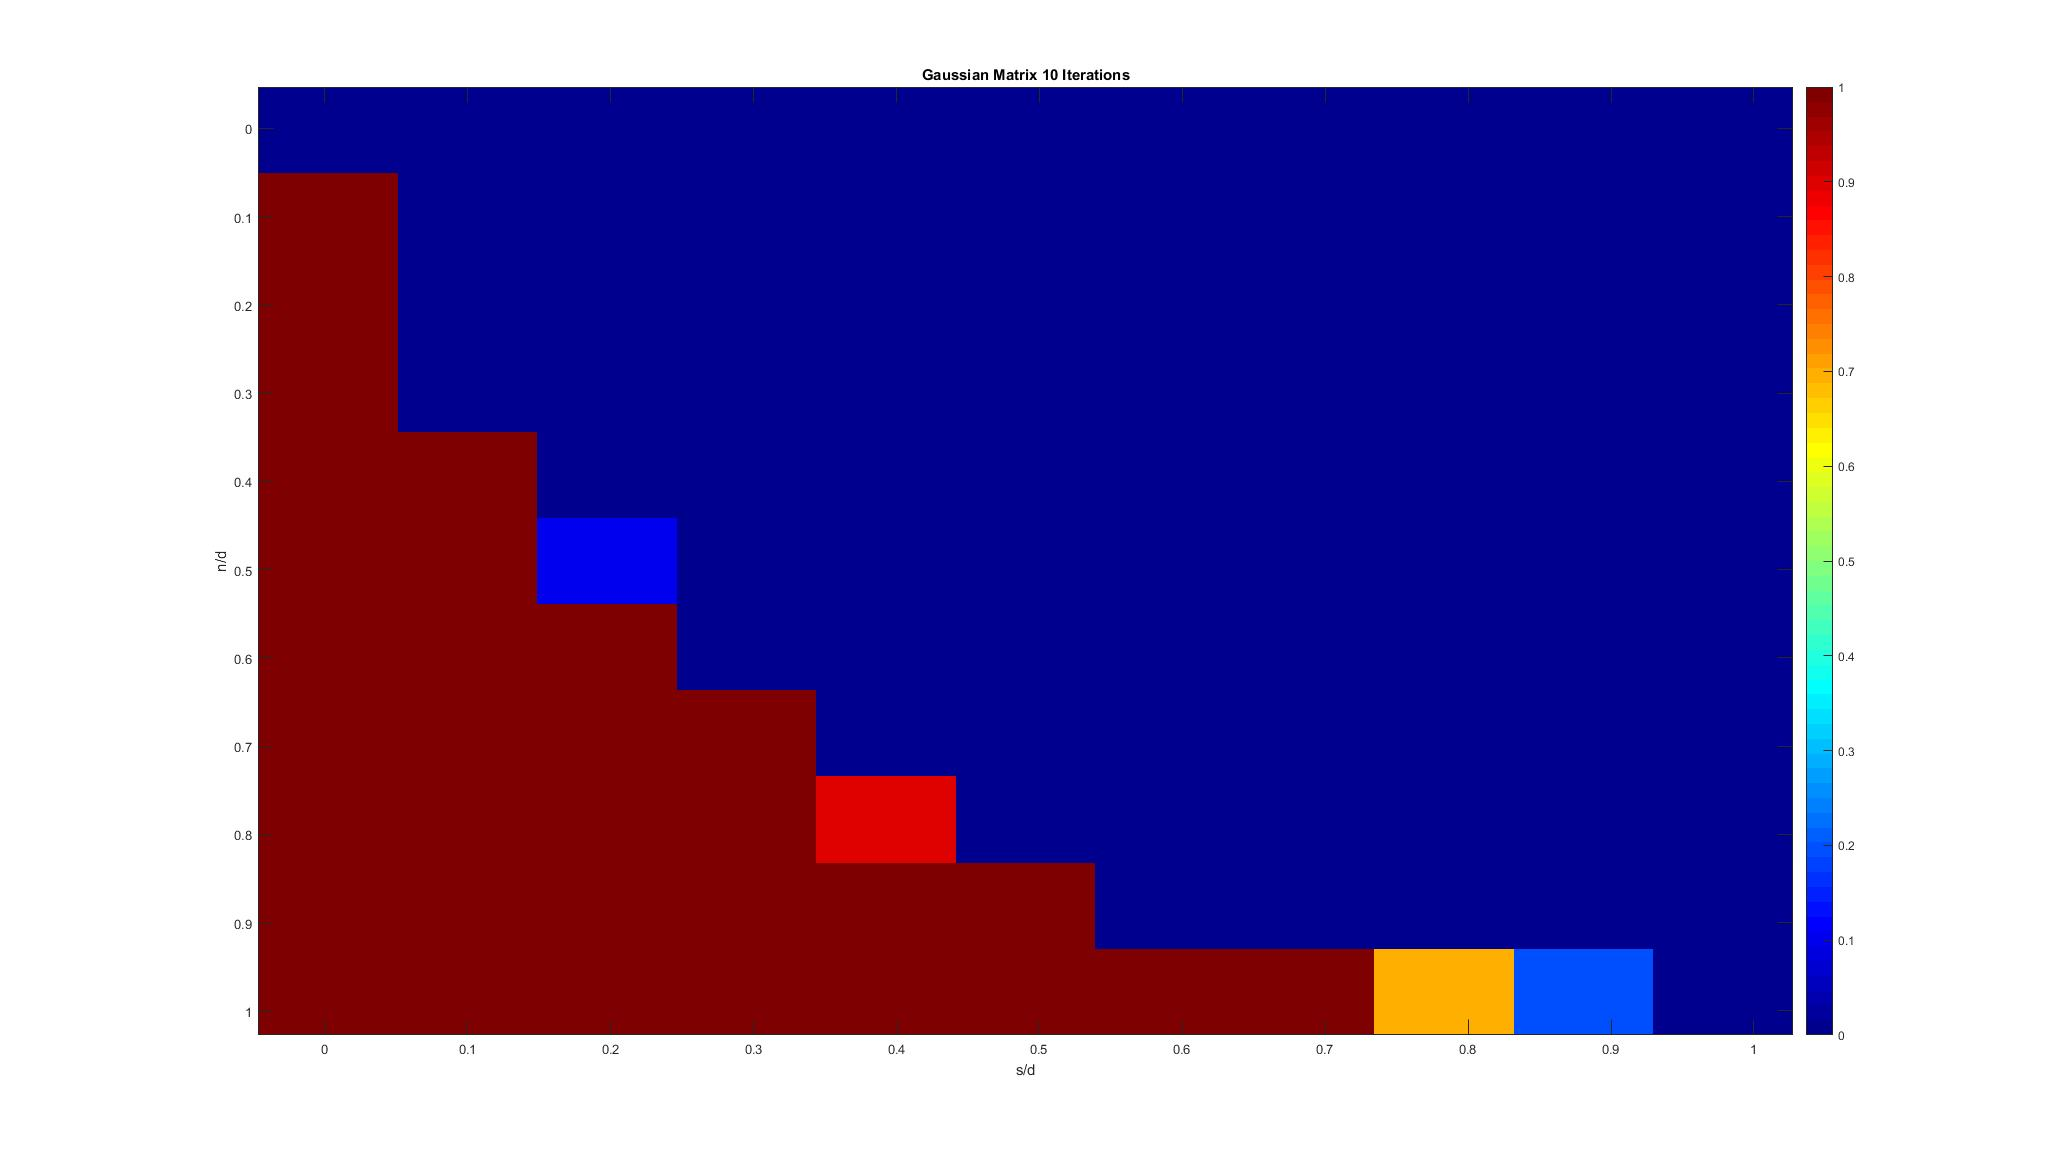
\includegraphics[width=0.9\textwidth]{gaussian.jpg}
        \captionof{figure}{Gaussian Matrix Probabilities}
      \end{center}

      \begin{center}
        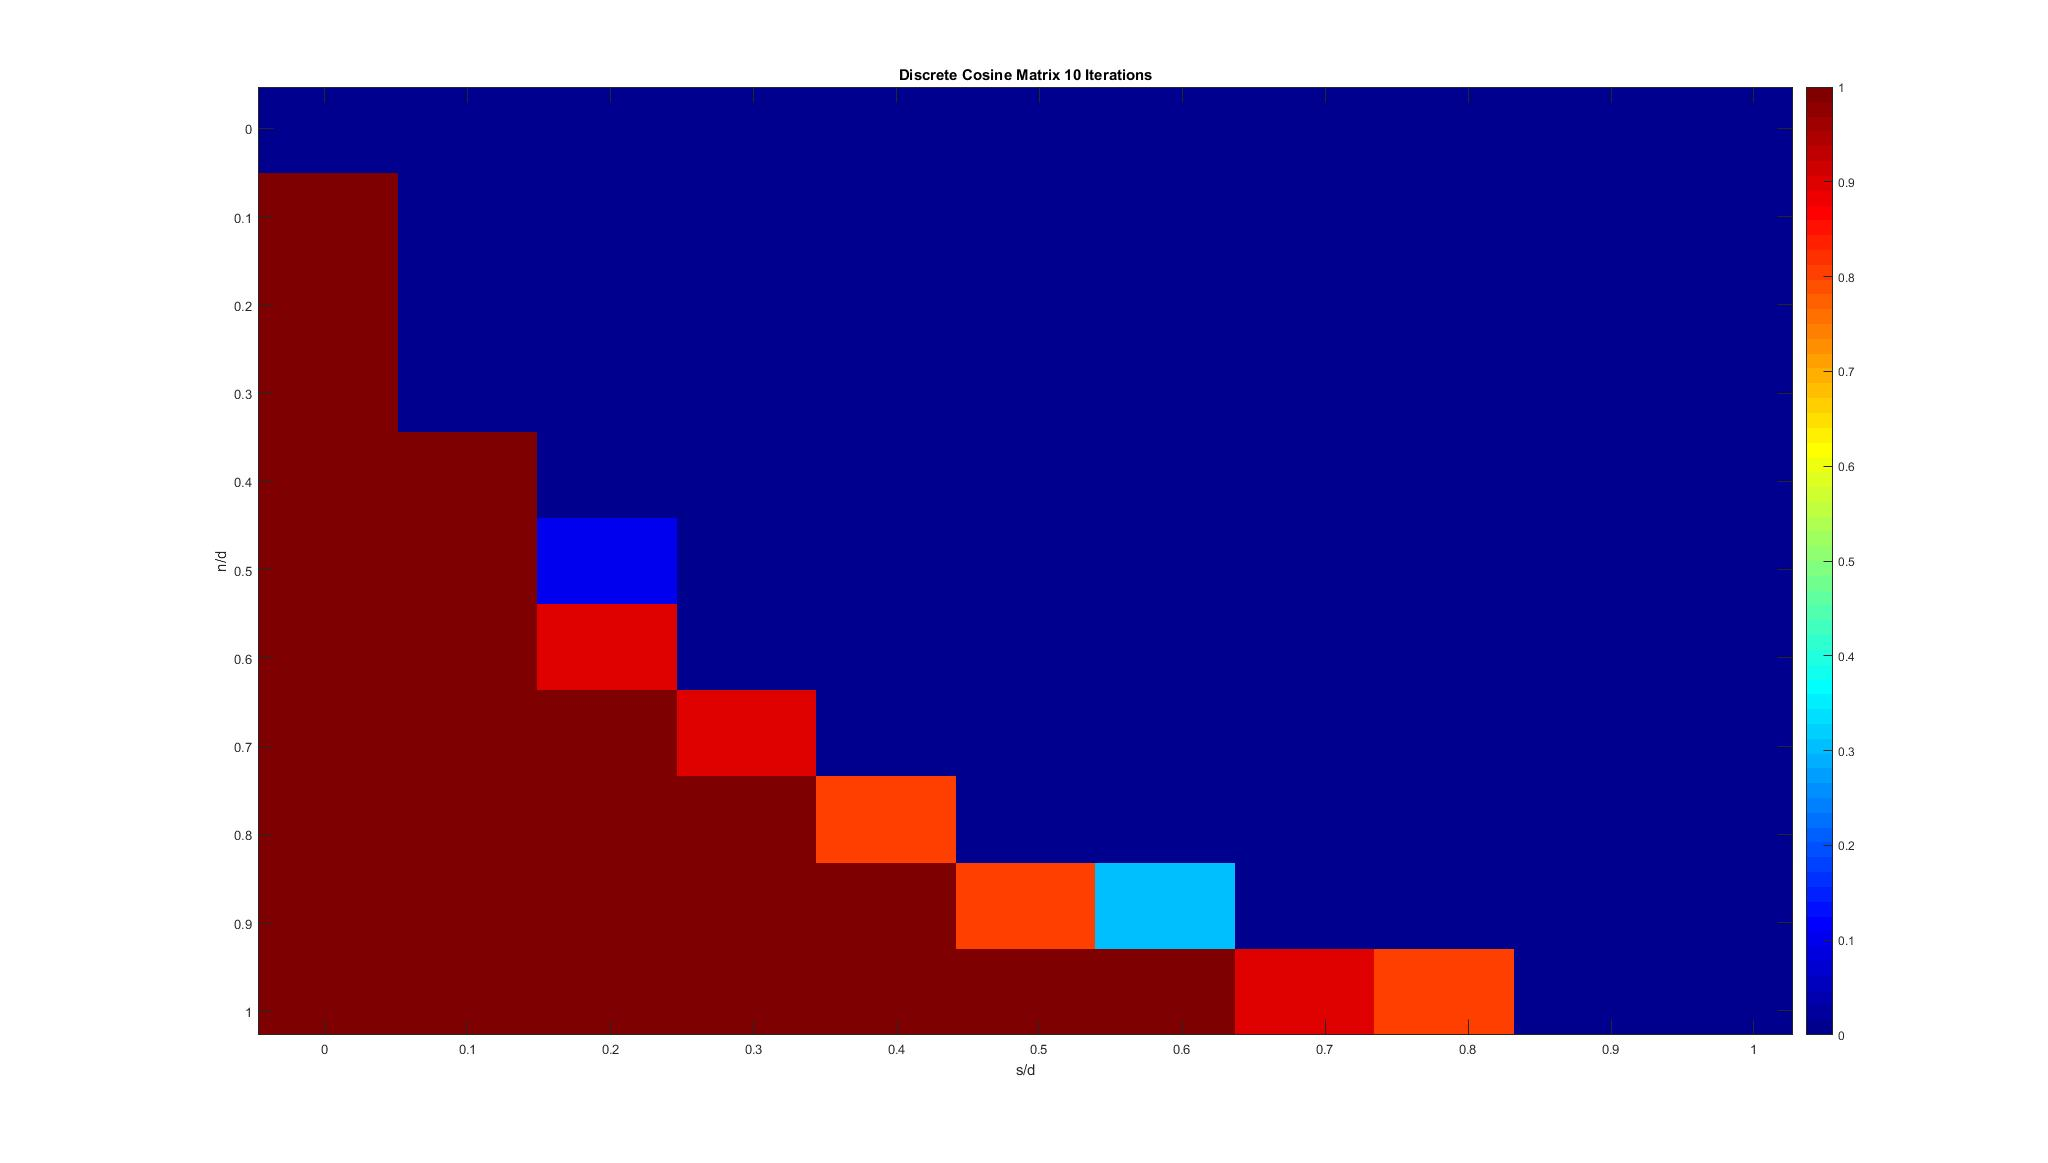
\includegraphics[width=0.9\textwidth]{dct.jpg}
        \captionof{figure}{Discrete Cosine Transform Matrix Probabilities}
      \end{center}

      \begin{center}
        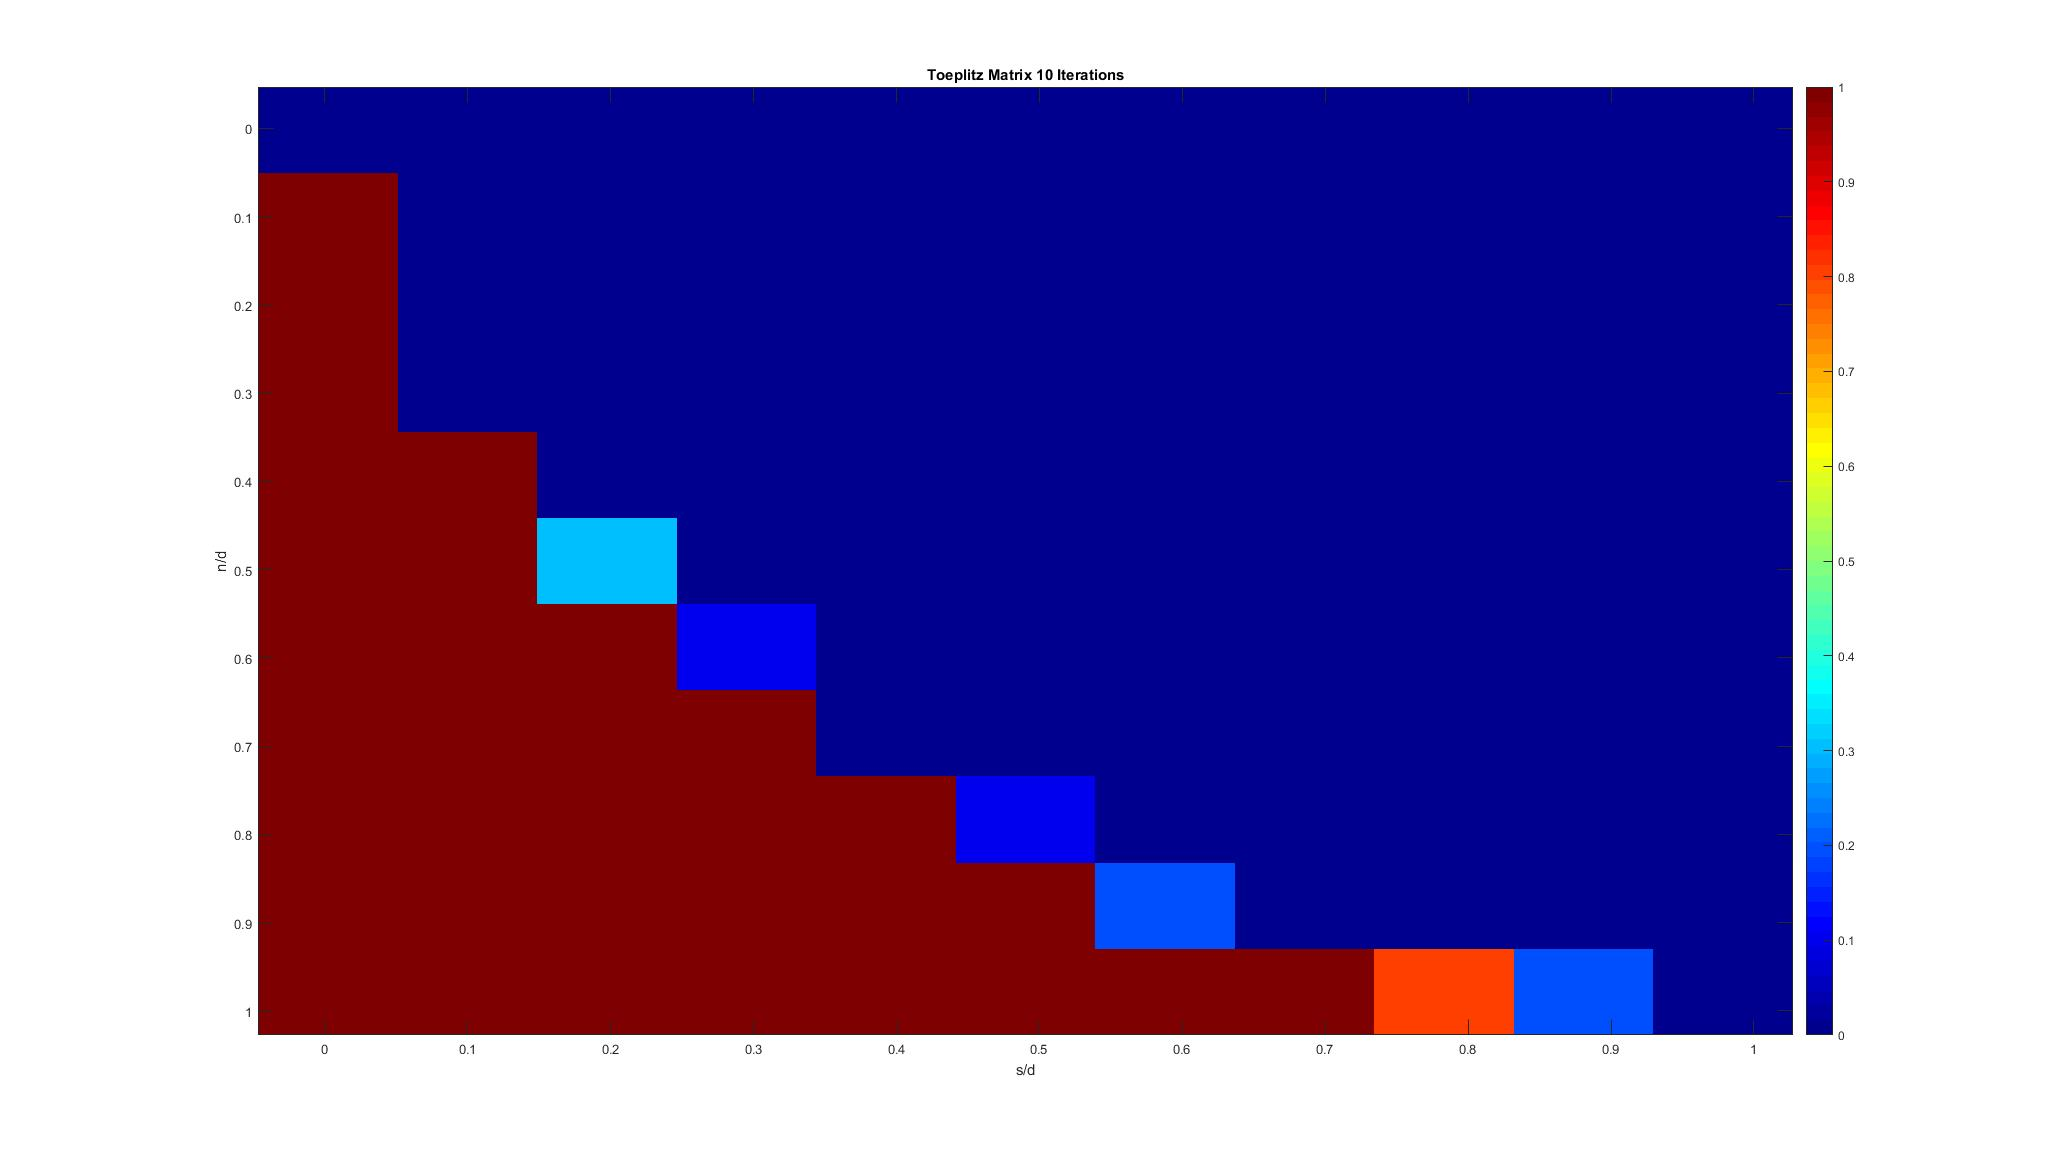
\includegraphics[width=0.9\textwidth]{toep.jpg}
        \captionof{figure}{Toeplitz Matrix Probabilities}
      \end{center}

      \textbf{Code Appendix}

      \begin{lstlisting}[style=Matlab-editor, basicstyle=\scriptsize]
        clear;
        clc;

        d = 512;
        iterations = 10;
        % Keep track of probability of success for pair (n,s)
        success = zeros(floor(d/50)+1, floor(d/50)+1);

        for i=1:iterations
            for s=1:50:d
                for n=1:50:d
                    % Change the random method
                    X = SubDCT_Phi(n,d);

                    % Generate random beta and zero the first d-s entries
                    beta = randn(d, 1);
                    beta(1:(d-s),1)=0;

                    Y = X*beta;

                    sol = l1eq_pd(0*beta, X, 0*X, Y);

                    % Check if solution is close to original beta
                    if(norm(l1eq_pd(0*beta, X, 0*X, Y) - beta) < 0.01)
                        success(floor(n/50) + 1, floor(s/50) + 1) = success(floor(n/50) + 1, floor(s/50) + 1) + 1;
                    end
                end
            end
        end

        dlmwrite('dct.txt', success/iterations)
        colormap('jet')
        imagesc((1:50:d)/d,(1:50:d)/d, success/iterations)
        colorbar
        xlabel('s/d')
        ylabel('n/d')
        title('Discrete Cosine Matrix 10 Iterations')
      \end{lstlisting}
  \end{enumerate}
\end{answer}

\end{document}